%\documentclass[11pt]{article}
\title{\textbf{CV Homework 5}}
\author{Eric Feuvrier Danziger\\
		}
\date{}
%\usepackage{graphicx}
%\usepackage{float}
%\usepackage{amsmath}
\begin{document}


\section*{1.1}
$p' = \begin{bmatrix}
0 \\
0 \\
1 \\
\end{bmatrix}$\\$\\
$p^T = [0 0 1]$
$F = 
\begin{bmatrix}
F_{21} F_{22} F_{23} \\
F_{31} F_{32} F_{33} \\
\end{bmatrix}$
The equation for converting points in two cameras based on the fundamental matrix is $p^T*F*p’ = 0$\\
This means \\
$p^T * F = [F_{31} F_{32} F_{33}]$\\
This times p’ is 
$ [F_{31} F_{32} F_{33}] * \begin{bmatrix}
0 \\
0 \\
1 \\
\end{bmatrix}$ \\
The result is $F_{33} = 0$
\section*{1.2}





$A^TA$ is the Hessian. It is the sum of all pairs of gradients\\
$\begin{bmatrix}
\sum{dxdx} \sum{dxdy}\\
\sum{dxdy} \sum{dydy}\\
\end{bmatrix}$\\
$A^TA$ has to be invertible so that the $\Delta{p}$ can be calculated.\\

\section*{1.3 Car Tracking}
The rectangle is only translated, and tracks the car as follows:
%\begin{figure}[H]
%\centering
%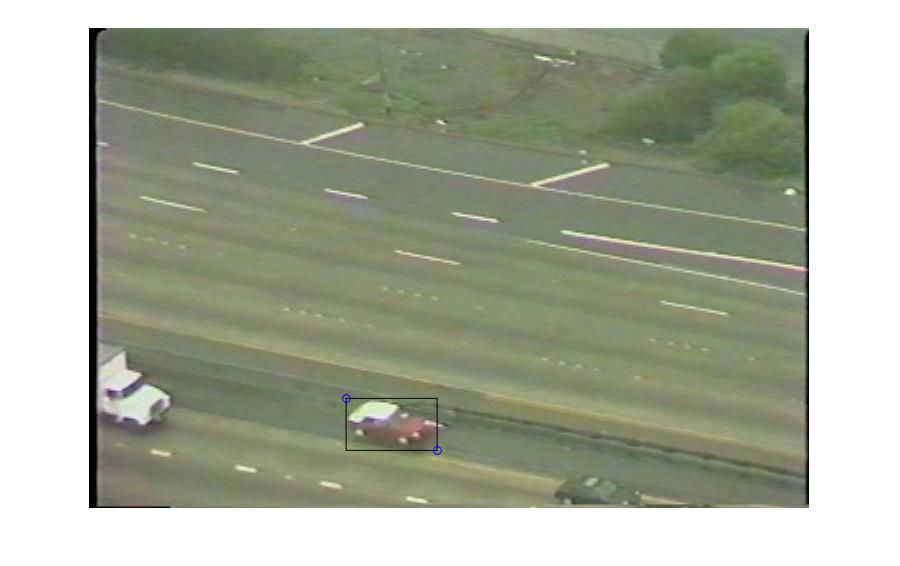
\includegraphics[width=90mm]{carFrame20.jpg}
%\caption{ 20 }
%\end{figure}

%\begin{figure}[H]
%\centering
%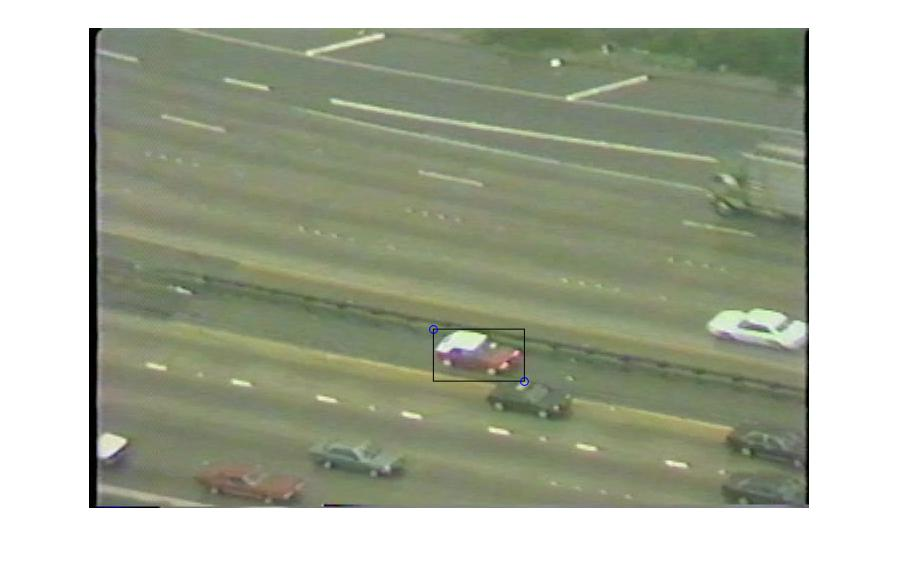
\includegraphics[width=90mm]{carFrame50.jpg}
%\caption{ 50 }
%\end{figure}

%\begin{figure}[H]
%\centering
%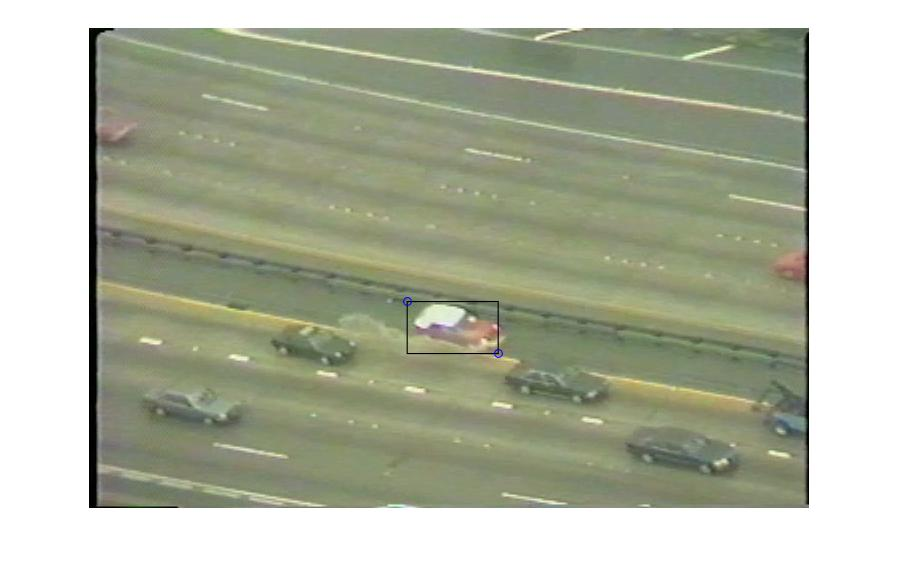
\includegraphics[width=90mm]{carFrame100.jpg}
%\caption{ 100 }
%\end{figure}


\section*{1.4 Failure Modes for Translating L-K Tracking}
There are several reasons the tracker could fail. The primary is occlusion, where the object being tracked is lost and the tracker then templates a new object. 

Even partial occlusion could cause problems. A possible solution to this is to implement a more robust method of updating the template than just every frame - mabe by verifying that there are greater than some number of feature matches with the last few templates and the current guess. 

Another possibility is low frame rate, where the car translates too far for the tracker to update, depending on if the tracker is constrained on number of iterations. 
\end{document}
